%The infrared colors[W1($\sim 3.4\mu$m)-W2 ($\sim 4.5\mu$m)] of CLAGNs 
  
%The discovery of changing-look active galactic nuclei (CLAGNs) in recent years with rapid change of optical broad emission lines and/or change of line-of-sight column densities challenges the AGN unified model. The origin of changing-look phenomena is still unclear, but there is some evidence supporting the scenario of the change of the intrinsic accretion rate as the explanation of changing-look phenomena in the most of cases. The emission and variability from mid-infrared (MIR) band are good tracers of the activity of nuclei. We search a sample of CLAGNs with significant variability and study their intrinsic amplitude of variability ($\sigma_m$) in MIR band. There is significant stronger MIR variability in optical CLAGNs than that of X-ray CLAGNs, low-luminosity AGN (LLAGNs), and luminous quasi-stellar objects (QSOs). The MIR Eddington scaled luminosity distribution of CLAGNs is centred between quiescent LLAGNs and luminous QSOs. The mean Eddington scaled MIR luminosity $\sim 0.5$ per cent is close to the critical value of state transition between a radiatively inefficient accretion flow and a thin accretion disk. The distributions of MIR luminosity and color ($W1$-$W2$) suggest that CLAGNs are in transitional accretion state with extreme variability. Besides, there is a tight correlation between dust echo time lag and the luminosity ($\tau - L$) for CLAGNs, which again confirms the influence of accretion process.

%luminous galaxies that powered by matter accretion onto the supermassive black hole (SMBH) in the center of galaxies. Based on the brightness of nuclei and excitation of emission lines, the main subclasses of AGNs include nearby Seyfert galaxies \citep{1943ApJ....97...28S} with bright nuclei and high-excitation emission lines, low-ionization nuclear emission-line regions \citep[LINERs; e.g.,][]{2014ARA&A..52..589H}, and extremely luminous and distant quasi-stellar objects (QSOs, or quasars).  Based on the appearance or disappearance of broad emission lines, AGN are divided into two classes.  One is type 1 AGN with both broad lines ($>$ 1000 $ \rm{km}\, \rm{s}^{-1}$) and narrow lines ($<$ 1000 $ \rm{km}\, \rm{s}^{-1}$), and another is type 2 AGN with only narrow lines. The sub-classes are classified based on the strength of broad H$\alpha$ lines and broad H$\beta$ line \citep[see ][]{1976MNRAS.176P..61O,1981ApJ...249..462O}. Type 1.5/1.8/1.9 AGN has broad H$\alpha$ lines and comparable/weak/undetectable broad H$\beta$ lines.

%Different type of AGNs show much different continuum, which are mainly regulated by the evolution of accretion process and jet. 
%AGN unification is proposed to explain different kinds of AGNs \citep[e.g.,][and references therein]{1993ARA&A..31..473A,2015ARA&A..53..365N}, which is described in a general picture with two parameters: the inclination to the line of sight and the luminosity of source. AGNs with higher Eddington ratio $L_\mathrm{AGN}/L_\mathrm{Edd} \ge 0.01$ (such as QSOs and Seyfert galaxies) are efficient accretors. The mechanism of energy output of bright AGNs are thought to come from matter accretion through an optically thick and geometrically thin accretion disk \citep[SSD;][]{1973A&A....24..337S}.  Low-luminosity AGNs \citep[LLAGNs;e.g.,][]{2008ARA&A..46..475H} with much lower Eddington ratio luminosity are in radiatively inefficient accretion mode, where the thin disk is  thought to be truncated in the inner regions by a geometrically thick advection-dominated accretion flow or radiatively inefficient accretion flows\citep[ADAF/RIAF; e.g.,][and references therein]{2014ARA&A..52..529Y}. 


% X-ray spectra transit between Compton thick (e.g., hydrogen equivalent column density, $N_\mathrm{H}$ above $\sim 10^{24}\,\mathrm{cm}^{-2}$) and Compton thin \citep[e.g., $N_\mathrm{H} \sim  10^{22-23}\,\mathrm{cm}^{-2}$; see ][]{2003MNRAS.342..422M}. Optical CLAGNs are also named since 2010s through the optical spectroscopic confirmation that the AGN type change based on the appearance/disappearance of broad-emission lines within years \citep[e.g.,][]{2014ApJ...796..134D,2014ApJ...788...48S,2020ApJ...890L..29A,2020ApJ...901....1W}, even months \citep[e.g.,][]{2019MNRAS.487.4057K,2019ApJ...883...94T}. There has been some systematic search for CLAGNs using multi-epoch optical spectra \citep[e.g.,][]{2018ApJ...862..109Y,2021MNRAS.503.2583S,2021A&A...650A..33P} and the number of CLAGNs is growing.


%In the orientation-based unified model, type 1 AGN is face-on view with broad-emission lines region (BLR) visible to observer, while type 2 AGN is edge-on viewed with BLR blocked by the putative torus surrounding the BH. Source type should keep unchanged during short timescale under this scenario. However, changing-look AGNs (CLAGNs, hereafter) with optical broad emission line or X-ray spectrum variation have been discovered in recent years. The term ``changing-look" is firstly used to describe the X-ray CLAGNs, whose X-ray spectra transit between Compton thick (e.g., hydrogen equivalent column density, $N_\mathrm{H}$ above $\sim 10^{24}\,\mathrm{cm}^{-2}$) and Compton thin \citep[e.g., $N_\mathrm{H} \sim  10^{22-23}\,\mathrm{cm}^{-2}$; see ][]{2003MNRAS.342..422M}. Optical CLAGNs are also named since 2010s through the optical spectroscopic confirmation that the AGN type change based on the appearance/disappearance of broad-emission lines within years \citep[e.g.,][]{2014ApJ...796..134D,2014ApJ...788...48S,2020ApJ...890L..29A,2020ApJ...901....1W}, even months \citep[e.g.,][]{2019MNRAS.487.4057K,2019ApJ...883...94T}. There has been some systematic search for CLAGNs using multi-epoch optical spectra \citep[e.g.,][]{2018ApJ...862..109Y,2021MNRAS.503.2583S,2021A&A...650A..33P} and the number of CLAGNs is growing.

%%%Such a change could either occur in tidal disruption events\citep{2015ApJ...800..144L,2021MNRAS.500L..57Z}, disks with tidal interactions in SMBH binaries \citep{2020A&A...643L...9W}, Czerny disk instability model \citep{2020A&A...641A.167S}, etc.
%{\color{red}the gradual variation of accretion rate or AGNs experiencing a stochastic extreme change on accretion (references, Wang Jianmin binary BH , Czerny disk instability model ...).}





%The mechanism of the ``changing-look" is still unclear. One scenario is that broad lines change with variable obscuration, such as obscuring material moving in or out from our line of sight\citep[e.g.,][]{2013MNRAS.436.1615M,2014MNRAS.443.2862A,2015ApJ...815...55R,2018MNRAS.481.2470T,2019ApJ...887...15W} and the intrinsic emission is roughly unchanged. Only a small portion of sources might be explained in this scenario. \citet{2017ApJ...846L...7S} reports the significant mid-infrared (MIR) variability with the type transition of several optical CLAGNs. The variable obscuration scenario is ruled out since the crossing time for obscuration is much longer than the MIR variability timescale. Another promising scenario is that the AGN type evolves with the variation of intrinsic radiation such as accretion rate change \citep[e.g.,][]{1984MNRAS.211P..33P,2014MNRAS.438.3340E}, which is supported by low $N_\mathrm{H}$\citep[e.g.,][]{2016A&A...593L...9H} and almost unchanged polarization degree measurements \citep[e.g.,][]{2019sf2a.conf..509M}. There is also consistent variation of AGN types with luminosity in X-ray \citep[e.g.,][]{2021MNRAS.508..144G}, and MIR \citep[e.g.,][]{2017ApJ...846L...7S,2018ApJ...864...27S} band. Multi-wavelength variability is expected in CLAGNs and search for CLAGN candidates based on infrared \citep[][]{2020ApJ...889...46S} or hard X-ray \citep[][]{2021AIPC.2319d0007H} variability has been conducted. Changing-look quasars \citep[e.g.,][]{2015ApJ...800..144L,2021PASJ...73..122N}, changing-look LINERs \citep{2019ApJ...883...31F}, and even a changing-look Blazar \citep{2021ApJ...913..146M} represent the extreme variability and rapid type transition over an wide luminosity range of AGNs. CLAGNs with luminosity variation crossing $\sim1$ per cent Eddington ratio might be in the transitional accretion state between quiescent LLAGNs and active QSOs, which might be tested through statistical study. Besides, recent studies show that changing-look Seyferts galaxies hosts primarily reside in the green valley between spiral-like star-forming galaxies and dead elliptical galaxies \citep{2021ApJ...907L..21D,2021ApJ...915...63L}, whereas changing-look quasars hosts reside in the star-forming main sequence \citep{2021ApJ...915...63L}. The host galaxies of CLAGNs might also experience co-evolution through episodic bursts of accretion activity with changing-look LINERs, changing-look Seyferts, and changing-look quasars in different accretion mode. CLAGNs with large amplitude variation of luminosity provide us opportunity to study the possible transition of accretion mode in individual sources. The X-ray spectra evolution with a `q'-shape of the hardness-intensity diagram found in CLAGNs \citep[e.g., NGC 1566;][]{2021MNRAS.507..687J} are similar to the state transitions in black hole X-ray binaries. The correlation between hardness ratio or the photon index ($\Gamma$) from X-ray spectrum and X-ray luminosity \citep[e.g., Mrk 1018;][]{2018MNRAS.480.3898N,2021MNRAS.506.4188L} and the bolometric luminosity distribution \citep[e.g., NGC 2992;][]{2021MNRAS.508..144G} show significant discrepancy when optical CLAGNs are type 1 and type 2 with a critical Eddington ratio $\sim 1$ per cent. The evolution of BLR might be regulated by the transition of accretion mode. Besides, there is also strong X-ray spectral evolution with variable $N_\mathrm{H}$ \citep[e.g., NGC 1365;][]{2021RAA....21..199L} in X-ray CLAGNs. 






%Whether the optical type change and X-ray spectral evolution in CLAGNs are regulated by the same process is still an issue. The emission and color variability from MIR band are good tracers for CLAGNs with intrinsic variation \citep[e.g.,][]{2018ApJ...862..109Y}. The MIR variability is driven by the intrinsic variation such as accretion rate change in the reprocessing scenario. When the optical/UV emission from accretion disk changes, the reprocessed IR emission would respond to the variation as the variation signal travels to the torus at the speed of light. The MIR light curves of several optical CLAGNs shifted backward a few of years match well with optical variation pattern, showing evidence of the dust echo response to the intrinsic accretion variation \citep{2017ApJ...846L...7S}. Dust reverberation that measures the time lag between MIR band and optical or hard X-ray band is an effective method to estimate the size of torus. This method has been extensively applied in quasars \citep[e.g.,][]{2019ApJ...886...33L}, Seyfert 1s \citep[e.g.,][]{2014ApJ...788..159K,2019ApJ...886...33L,2021MNRAS.501.3905M} and type 2 AGN \citep[e.g.,][]{2020MNRAS.495.2921N} and some CLAGNs are included \citep[e.g.,][]{2014ApJ...788..159K,2014ApJ...788...48S,2019ApJ...886...33L,2020MNRAS.491.4615K,2021ApJ...912..126L}. 

%In this work, we systematically study the MIR band variability of a CLAGN sample and compare them with a sample of LLAGNs and QSOs. We estimate the dust reverberation time lag ($\tau$) between optical V band and MIR $W$1 band of several CLAGNs using multi-wavelength observations to study the correlation between dust reverberation time lag ($\tau$) and bolometric luminosity ($L_\mathrm{bol}$). This paper is organized as follows. We describe the CLAGN sample and MIR {\it WISE} data in \autoref{sec:sample}. The results of MIR variability, color, and luminosity for CLAGNs are shown in \autoref{sec:mir_var_col_lum}. We present the $\tau$-$L_\mathrm{bol}$ correlation of CLAGNs in  \autoref{sec:tau-L}. Conclusion and discussion are presented in \autoref{sec:dis}. Throughout this work, we adopt a flat $\Lambda-$CDM cosmological model with $H_0$=70 km s$^{-1}$ Mpc $^{-1}$, $\Omega_{m}$=0.27, and $\Omega_{\Lambda}=0.73 $.


%We collect over one hundred of CLAGNs from literature. 13 of them are X-ray CLAGNs with $N_\mathrm{H}$ variation from X-ray spectrum \citep[e.g.,][]{2003MNRAS.342..422M,2005MNRAS.356..295G,2012MNRAS.421.1803M,2013MNRAS.428.2516B,2016ApJ...820....5R,2020MNRAS.499.5396J,2021MNRAS.507..687J}. The others are optical CLAGNs with optical type change between type 1 (type 1--type 1.8) and type 2 (type 1.9--type 2). Some sources (e.g., ESO 362-G18, IRAS 23226-3843, NGC 2992, NGC 4151, NGC 4395, and NGC 7582) with both optical type change and variable X-ray spectrum observed during different periods \citep[e.g.,][]{2003MNRAS.342..422M,2011MNRAS.417.2571N,2014MNRAS.443.2862A,2015ApJ...815...55R,2017A&A...603A..50B,2020A&A...638A..91K} are classified into optical CLAGNs. Around 119 of CLAGNs have central BH mass ($M_\mathrm{BH}$) measurements reported in literature. The BH mass measurements are based on kinematics method \citep[e.g.,][]{2003MNRAS.345.1057M}, reverberation mapping (RM) method \citep[e.g.,][]{2011MNRAS.410.1877S,2017ApJ...840...97F}, correlation between $M_\mathrm{BH}$ and bulge lumoninosity \citep[$L_\mathrm{bulge}$, e.g.,][]{2006AJ....131.1236D} and correlation between $M_\mathrm{BH}$ and the velocity dispersion $\sigma$ of the host galaxy \citep{2002ApJ...574..740T}.


%\subsection{{\it WISE} Data}
%In order to investigate the MIR variability and the intrinsic physics of CLAGNs, we use MIR data from \textit{Wide-field Infrared Survey Explorer}, which is launched on 2009, December 14 and performed all-sky survey in four bands, $W1$, $W2$, $W3$, and $W4$ at 3.4, 4.6, 12, and 22 $\mu$m until 2011\citep[\textit{WISE};][]{2010AJ....140.1868W} and the newly released Near-Earth Object WISE Reactivation mission\citep[\textit{NEOWISE};][]{2014ApJ...792...30M} which starts in 2013 with only $W1$ and $W2$ working. We use the \textit{AllWISE} multi-epoch photometry table and \textit{NEOWISE} single exposure (L1b) source table data retrieved from the NASA/IPAC Infrared Science Archive \footnote{\url{https://irsa.ipac.caltech.edu/Missions/wise.html}}. The \textit{AllWISE} and \textit{NEOWISE} data are screened to exclude the possible bad photometric measurements according to the following criteria:\\(1) Detection from good-quality frame sets\footnote{\url{http://wise2.ipac.caltech.edu/docs/release/neowise/expsup/sec2_3.html}}, with {frame quality score \texttt{qual\_frame}}$>$0, frame image quality score {\texttt{qi\_fact}}$>$0, South Atlantic Anomaly separation {\texttt{saa\_sep}}$>0$, and Moon masking flag {\texttt{moon\_masked}}=0.\\ (2) $W1$ $<$15 and $W2$ $<$13 mag, which approximately correspond to signal-noise-ratio SNR=10.\\ (3) The number of point spread function (PSF) components used in profile fit (\texttt{nb}$<$3) and frames are unaffected (\texttt{cc\textunderscore flags}=`0000') and are not actively de-blended \citep[na$=$0; see also][]{2019MNRAS.483.2362R}.
%w1rchi2<5,w2rchi2<5
%https://wise2.ipac.caltech.edu/docs/release/neowise/expsup/sec2_3.html


%Since \textit{NEOWISE} has covered much more and longer MIR observations than \textit{AllWISE}, only 70 sources with data points of \textit{NEOWISE} more than 20 are considered to make sure statistical significance. 
%We calculate the MIR variability for selected CLAGNs based on the {\it WISE} magnitude for each visit per half year. 

%{\color{red}The MIR variability, mean color, and MIR Eddington ratio for LLAGNs, CLAGNs, and QSOs samples are listed in \autoref{table_MIR_var_cor_lum}.}


%The MIR variability of optical CLAGNs are significant higher than that of X-ray CLAGNs, LLAGNs and QSOs. We plot the correlation between mean MIR color ($W1$-$W2$) and mean $L_\mathrm{W1}/L_\mathrm{Edd}$\, and the distribution of mean $W1$-$W2$ in \autoref{fig:color_ledd}. The distribution of Eddington-scaled $W$1 luminosity ($L_\mathrm{W1}/L_\mathrm{Edd}$) from the re-binned $W$1 data is shown in \autoref{fig:distribution_ledd}.  The mean log$L_\mathrm{W1}/L_\mathrm{Edd}$\, of $-2.33$ for CLAGNs corresponds to $\sim 0.47$ per cent Eddington scaled $W$1 luminosity. Optical CLAGNs show significant higher MIR variability, slightly lower Eddington luminosity ratio, and lower $W1$-$W2$ than X-ray CLAGNs. The MIR variability, mean color, and mean luminosity for LLAGNs, CLAGNs, and QSOs samples are presented in \autoref{table_MIR_var_cor_lum}. %The source information of CLAGNs is summarized in \autoref{source}.    

%where the MIR luminosity is derived from AB magnitude for $W1$ (\texttt{w1mpro} and \texttt{w1mpro\_ep}) and $W2$ (\texttt{w2mpro} and \texttt{w2mpro\_ep}) converted from Vega magnitude through $m_{\rm AB} = m_{\rm Vega} + \Delta m$, where $\Delta m$ are 2.699 and 3.339 for $W1$ and $W2$ bands, respectively



%We present the correlation between MIR $W$1 band variability $\sigma_{m W1}$ and mean Eddington scaled $W$1 luminosity $L_\mathrm{W1}/L_\mathrm{Edd}$\, and the distribution of $\sigma_{m W1}$ in \autoref{fig:var_ledd_hist}. The MIR luminosity is estimated from AB magnitude for $W1$ (\texttt{w1mpro} and \texttt{w1mpro\_ep}) and $W2$ (\texttt{w2mpro} and \texttt{w2mpro\_ep}) converted from Vega magnitude through $m_{\rm AB} = m_{\rm Vega} + \Delta m$, where $\Delta m$ are 2.699 and 3.339 for $W1$ and $W2$ bands, respectively. For comparison, we also plot a sample of quiescent LLAGNs from \citet{2009MNRAS.399..349G} with several sources which are classified as CLAGNs excluded and luminous QSOs from \citet{2007ApJ...667..131G}. 49 LLAGNs and 762 QSOs with at least 10 data points of \textit{NEOWISE} are included. The MIR variability of optical CLAGNs are significant higher than that of X-ray CLAGNs, LLAGNs and QSOs. We plot the correlation between mean MIR color ($W1$-$W2$) and mean $L_\mathrm{W1}/L_\mathrm{Edd}$\, and the distribution of mean $W1$-$W2$ in \autoref{fig:color_ledd}. The distribution of Eddington-scaled $W$1 luminosity ($L_\mathrm{W1}/L_\mathrm{Edd}$) from the re-binned $W$1 data is shown in \autoref{fig:distribution_ledd}.  The mean log$L_\mathrm{W1}/L_\mathrm{Edd}$\, of $-2.33$ for CLAGNs corresponds to $\sim 0.47$ per cent Eddington scaled $W$1 luminosity. Optical CLAGNs show significant higher MIR variability, slightly lower Eddington luminosity ratio, and lower $W1$-$W2$ than X-ray CLAGNs. The MIR variability, mean color, and mean luminosity for LLAGNs, CLAGNs, and QSOs samples are presented in \autoref{table_MIR_var_cor_lum}. The source information of CLAGNs is summarized in \autoref{source}. 


%The maximum variation magnitude $\Delta\,W1$ and $\Delta\,W2$ are estimated from the averaged light curve combining \textit{AllWISE} and \textit{NEOWISE} data. We find that the majority (59/70) of CLAGNs change more than $0.3$ mag for $\Delta\,W1$. And 6 of them are X-ray CLAGNs (NGC 4051, NGC 4388, NGC 4507, NGC 4939, NGC 7469, and PG 1535+547). The {\it WISE} light curves for those extreme variable sources are shown in \autoref{fig:X-CLAGN-lc}.  

%We average the {\it WISE} magnitude for each visit per half year. The errors are calculated by error propagation method.  The maximum variation magnitude $\Delta\,W1$ and $\Delta\,W2$ are estimated from the averaged light curve combining \textit{AllWISE} and \textit{NEOWISE} data. We find that the majority (59/70) of CLAGNs change more than $0.3$ mag for $\Delta\,W1$. And 6 of them are X-ray CLAGNs (NGC 4051, NGC 4388, NGC 4507, NGC 4939, NGC 7469, and PG 1535+547). The {\it WISE} light curves for those extreme variable sources are shown in \autoref{fig:X-CLAGN-lc}.  


%(see Appendix for more details for the data of each source)


%. The fitting result shows a slope of $0.29^{+0.04}_{-0.03}$ with a scatter of $0.02^{+0.04}_{-0.01}$ (solid line). The slope ($0.29^{+0.04}_{-0.03}$) of the $\tau$-$L_{bol}$ correlation is slightly lower than the slope ($0.47 \pm 0.06$) from the fitting of PG quasars (dashed line) in \citet[][]{2019ApJ...886...33L}.



%The physical connection and difference between optical and X-ray CLAGNs is still an issue. The majority of CLAGNs shows extreme MIR variability (see \autoref{fig:var_ledd_hist}). The extreme MIR variability in both optical and X-ray CLAGNs supports the variation of intrinsic accretion activity. Mean MIR variability of optical CLAGNs are significant stronger than that of LLAGNs and QSOs. With a limited sample of X-ray CLAGNs (only 13 sources), the mean MIR variability of X-ray CLAGNs are relatively lower than optical CLAGNs and similar to LLAGNs and QSOs. LLAGNs show galaxy-like MIR color, whereas the MIR color of QSOs are AGN-like. There is an obvious trend for CLAGNs that the mean color $W1$-$W2$ increases with the MIR luminosity \citep[see also][]{2017ApJ...846L...7S,2020ApJ...889...46S}. The color of X-ray CLAGN is more AGN-like, and the mean luminosity of X-ray CLAGNs is slightly higher than that of optical CLAGNs. The MIR color distribution CLAGNs is more similar to QSOs at higher luminosity range, while close to LLAGNs at lower luminosity. The distribution of MIR luminosity of CLAGNs is located between the quiescent LLAGNs and active QSOs (see \autoref{fig:distribution_ledd}). This suggests that CLAGNs are in a transitional state between LLAGNs and QSOs. The Eddington-ratio dependent ``changing-look'' phenomena have been found in some well-known CLAGNs through X-ray observation(e.g., Mrk 1018, NGC 1566, NGC 2992 and etc). The bolometric luminosity from X-ray spectral fitting cross the range of $\sim$ 1 per cent of Eddington luminosity during the ``changing-look'' events.  The mean MIR Eddington scaled luminosity $L_\mathrm{W1}/L_\mathrm{Edd} \sim $0.5 per cent is also close to the critical luminosity of accretion mode transition between ADAF and a thin accretion disk. As the intrinsic luminosity drops, the inner disk might transit into ADAF, reducing the supply of ionizing photons to excite the broad line or BLR are not sustainable when the intrinsic accretion rate declines below the critical value, and then AGN would change its optical type from type 1 to type 2 in the optical CLAGN. During the evolution of accretion disk in the X-ray CLAGN, disk-wind might form and influence the X-ray spectrum. Sources with $L_\mathrm{AGN}/L_\mathrm{Edd} \sim 0.01$ have the most extreme variability and are easily to experience the accretion mode transition, which might trigger the ``changing-look'' phenomena.  The MIR luminosity, variability, and color distribution also provide evidence that CLAGNs are in transitional accretion state with extreme variability. 


%It should be noted that 3 X-ray CLAGNs show no   

%The time lag between MIR and optical band is a good tracer of the dust echo response to the intrinsic accretion variation. The time lags between K band (2.19 $\mu$m) and V band of 6 CLAGNs (Mrk 590, NGC 3516, NGC 4051, NGC 4151, NGC 5548, and NGC 7469) in a sample of 17 Seyfert 1 AGNs have been reported \citep[see][]{2014ApJ...788..159K,2019ApJ...886...33L}. Except for Mrk 590, the time lag measurements from \citet[][]{2014ApJ...788..159K} and \citep{2019ApJ...886...33L} are almost consistent with average difference less than $10$ per cent. We present the time lags between $W$1 and V band of several CLANGs, in addition to the CLAGNs in the 17 Seyfert 1 AGNs sample. \citet[][]{2019ApJ...886...33L} reports that the inferred dust size ratios $R_\mathrm{K}$: $R_{W1}$: $R_{W2}$ are $0.6: 1: 1.2$. If we scale the reported $\tau_\mathrm{K}$ in \citet[][]{2014ApJ...788..159K} to $\tau_{W1}$ through $\tau_{W1}= \tau_\mathrm{K}/ 0.6$. The re-scaled $\tau_{W1}$ are roughly consistent with the direct measurements of $\tau_{W1}$ in this work. The time lags between MIR and optical V band and bolometric lumonisity in both optical/X-ray CLAGNs follow a tight $\tau$-L correlation (see \autoref{fig:tau_L}), further confirms that the dust echo response to the accretion process. The $\tau$-L correlation in CLAGNs supports the variable accretion scenario. 


%Mrk 590 & 43.84 & $ 33.8 \pm 4.20$ & O & \citet{2014ApJ...788..159K} \\
%NGC 3516 & 43.62 & $ 73.1 \pm 4.00$ & O & \citet{2014ApJ...788..159K} \\
%NGC 4051 & 42.66 & $ 16.5 \pm 0.60$ & X & \citet{2014ApJ...788..159K} \\
%NGC 4151 & 43.62 & $ 48.3 \pm 0.50$ & O & \citet{2014ApJ...788..159K} \\
%NGC 5548 & 43.87 & $ 60.9 \pm 0.30$ & O & \citet{2014ApJ...788..159K} \\
%NGC 7469 & 44.28 & $ 88.0 \pm 0.60$ & X & \citet{2014ApJ...788..159K} \\
%NGC 3516 & 43.84 & 53.6 & O & \citet{2019ApJ...886...33L} \\
%NGC 4051 & 42.88 & 12.9 & X & \citet{2019ApJ...886...33L} \\
%NGC 4151 & 43.84 & 52.2 & O & \citet{2019ApJ...886...33L} \\
%NGC 5548 & 44.07 & 50.5 & O & \citet{2019ApJ...886...33L} \\
%NGC 7469 & 44.45 & 56.1 & X & \citet{2019ApJ...886...33L} \\



As an example, we present the {\it WISE} light curves for those extreme variable X-ray CLAGNs in \autoref{fig:X-CLAGN-lc}. 
\begin{figure}
\centering
	% To include a figure from a file named example.*
	% Allowable file formats are eps or ps if compiling using latex
	% or pdf, png, jpg if compiling using pdflatex
	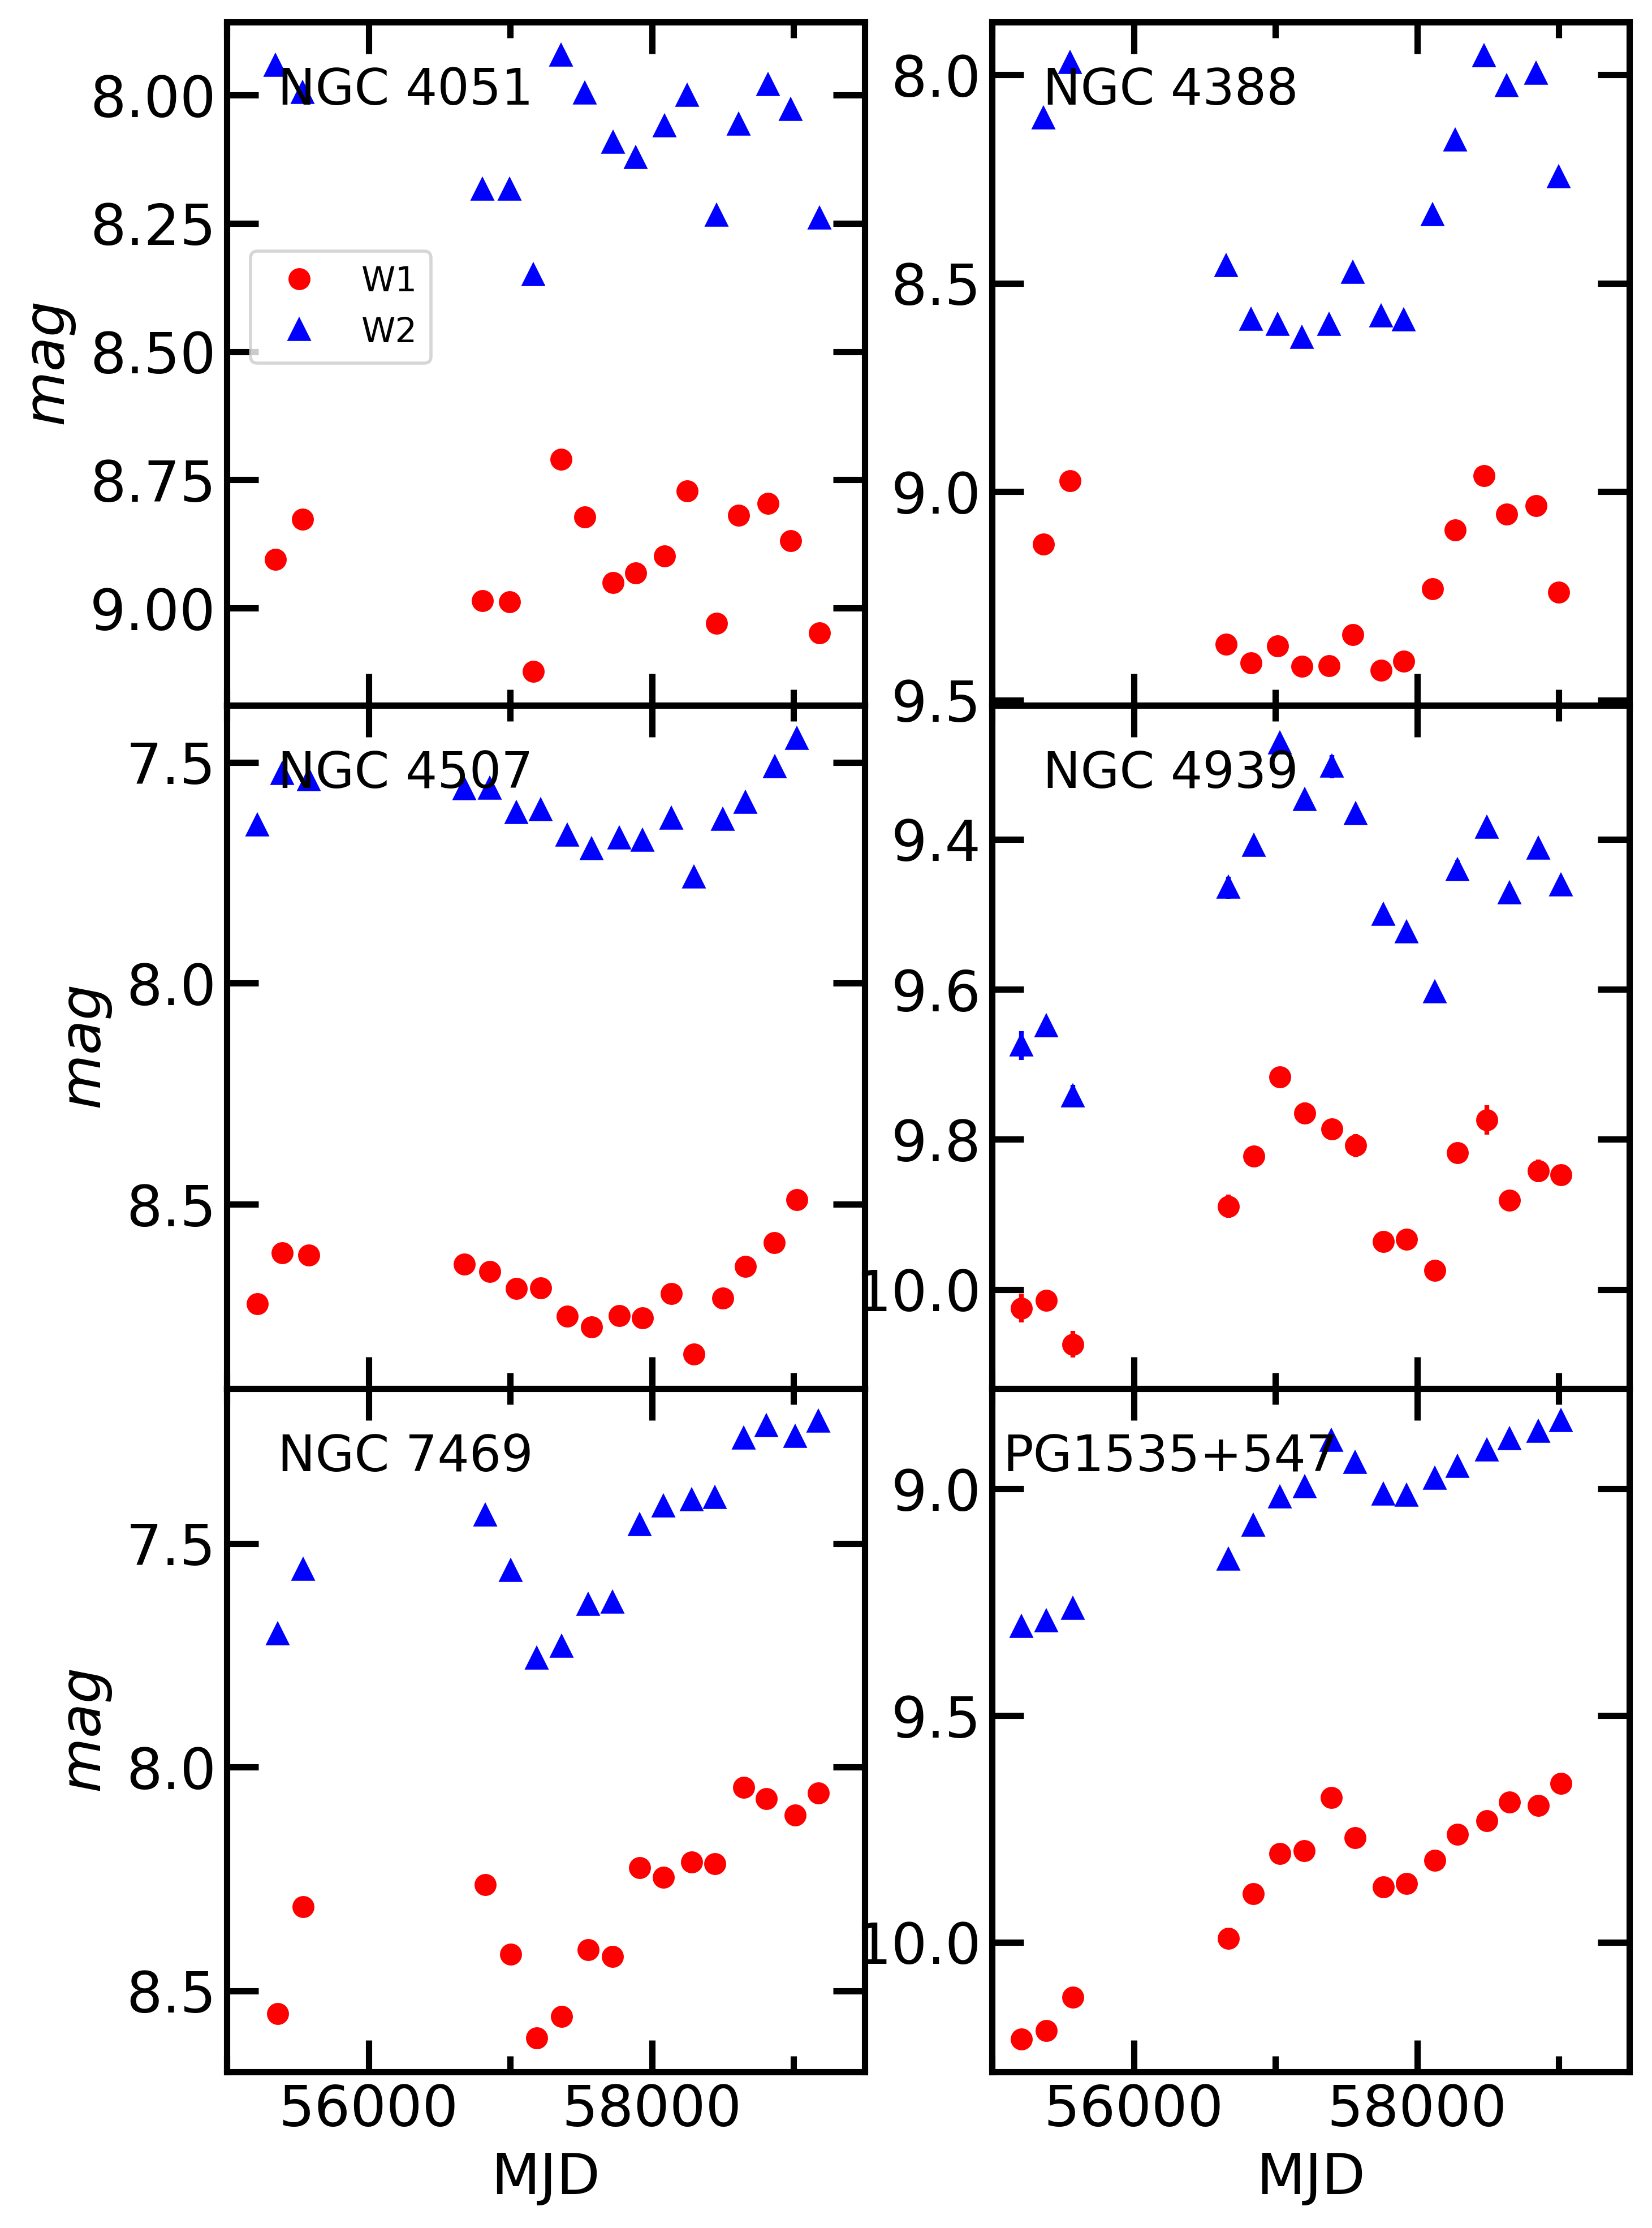
\includegraphics[width=0.6\textwidth]{pic/wisename_varX.png}
    \caption{{\it WISE} averaged light curves of highly variable X-ray CLAGNs with $\Delta\,W1$ more than $0.3$ mag. The errors are calculated by error propagation method. }
    \label{fig:X-CLAGN-lc}
\end{figure}

%All data obtained by {\it WISE} from 2010 and 2011 have been made public in the \textit{AllWISE} Data Release.


\begin{figure}
\centering
	% To include a figure from a file named example.*
	% Allowable file formats are eps or ps if compiling using latex
	% or pdf, png, jpg if compiling using pdflatex
	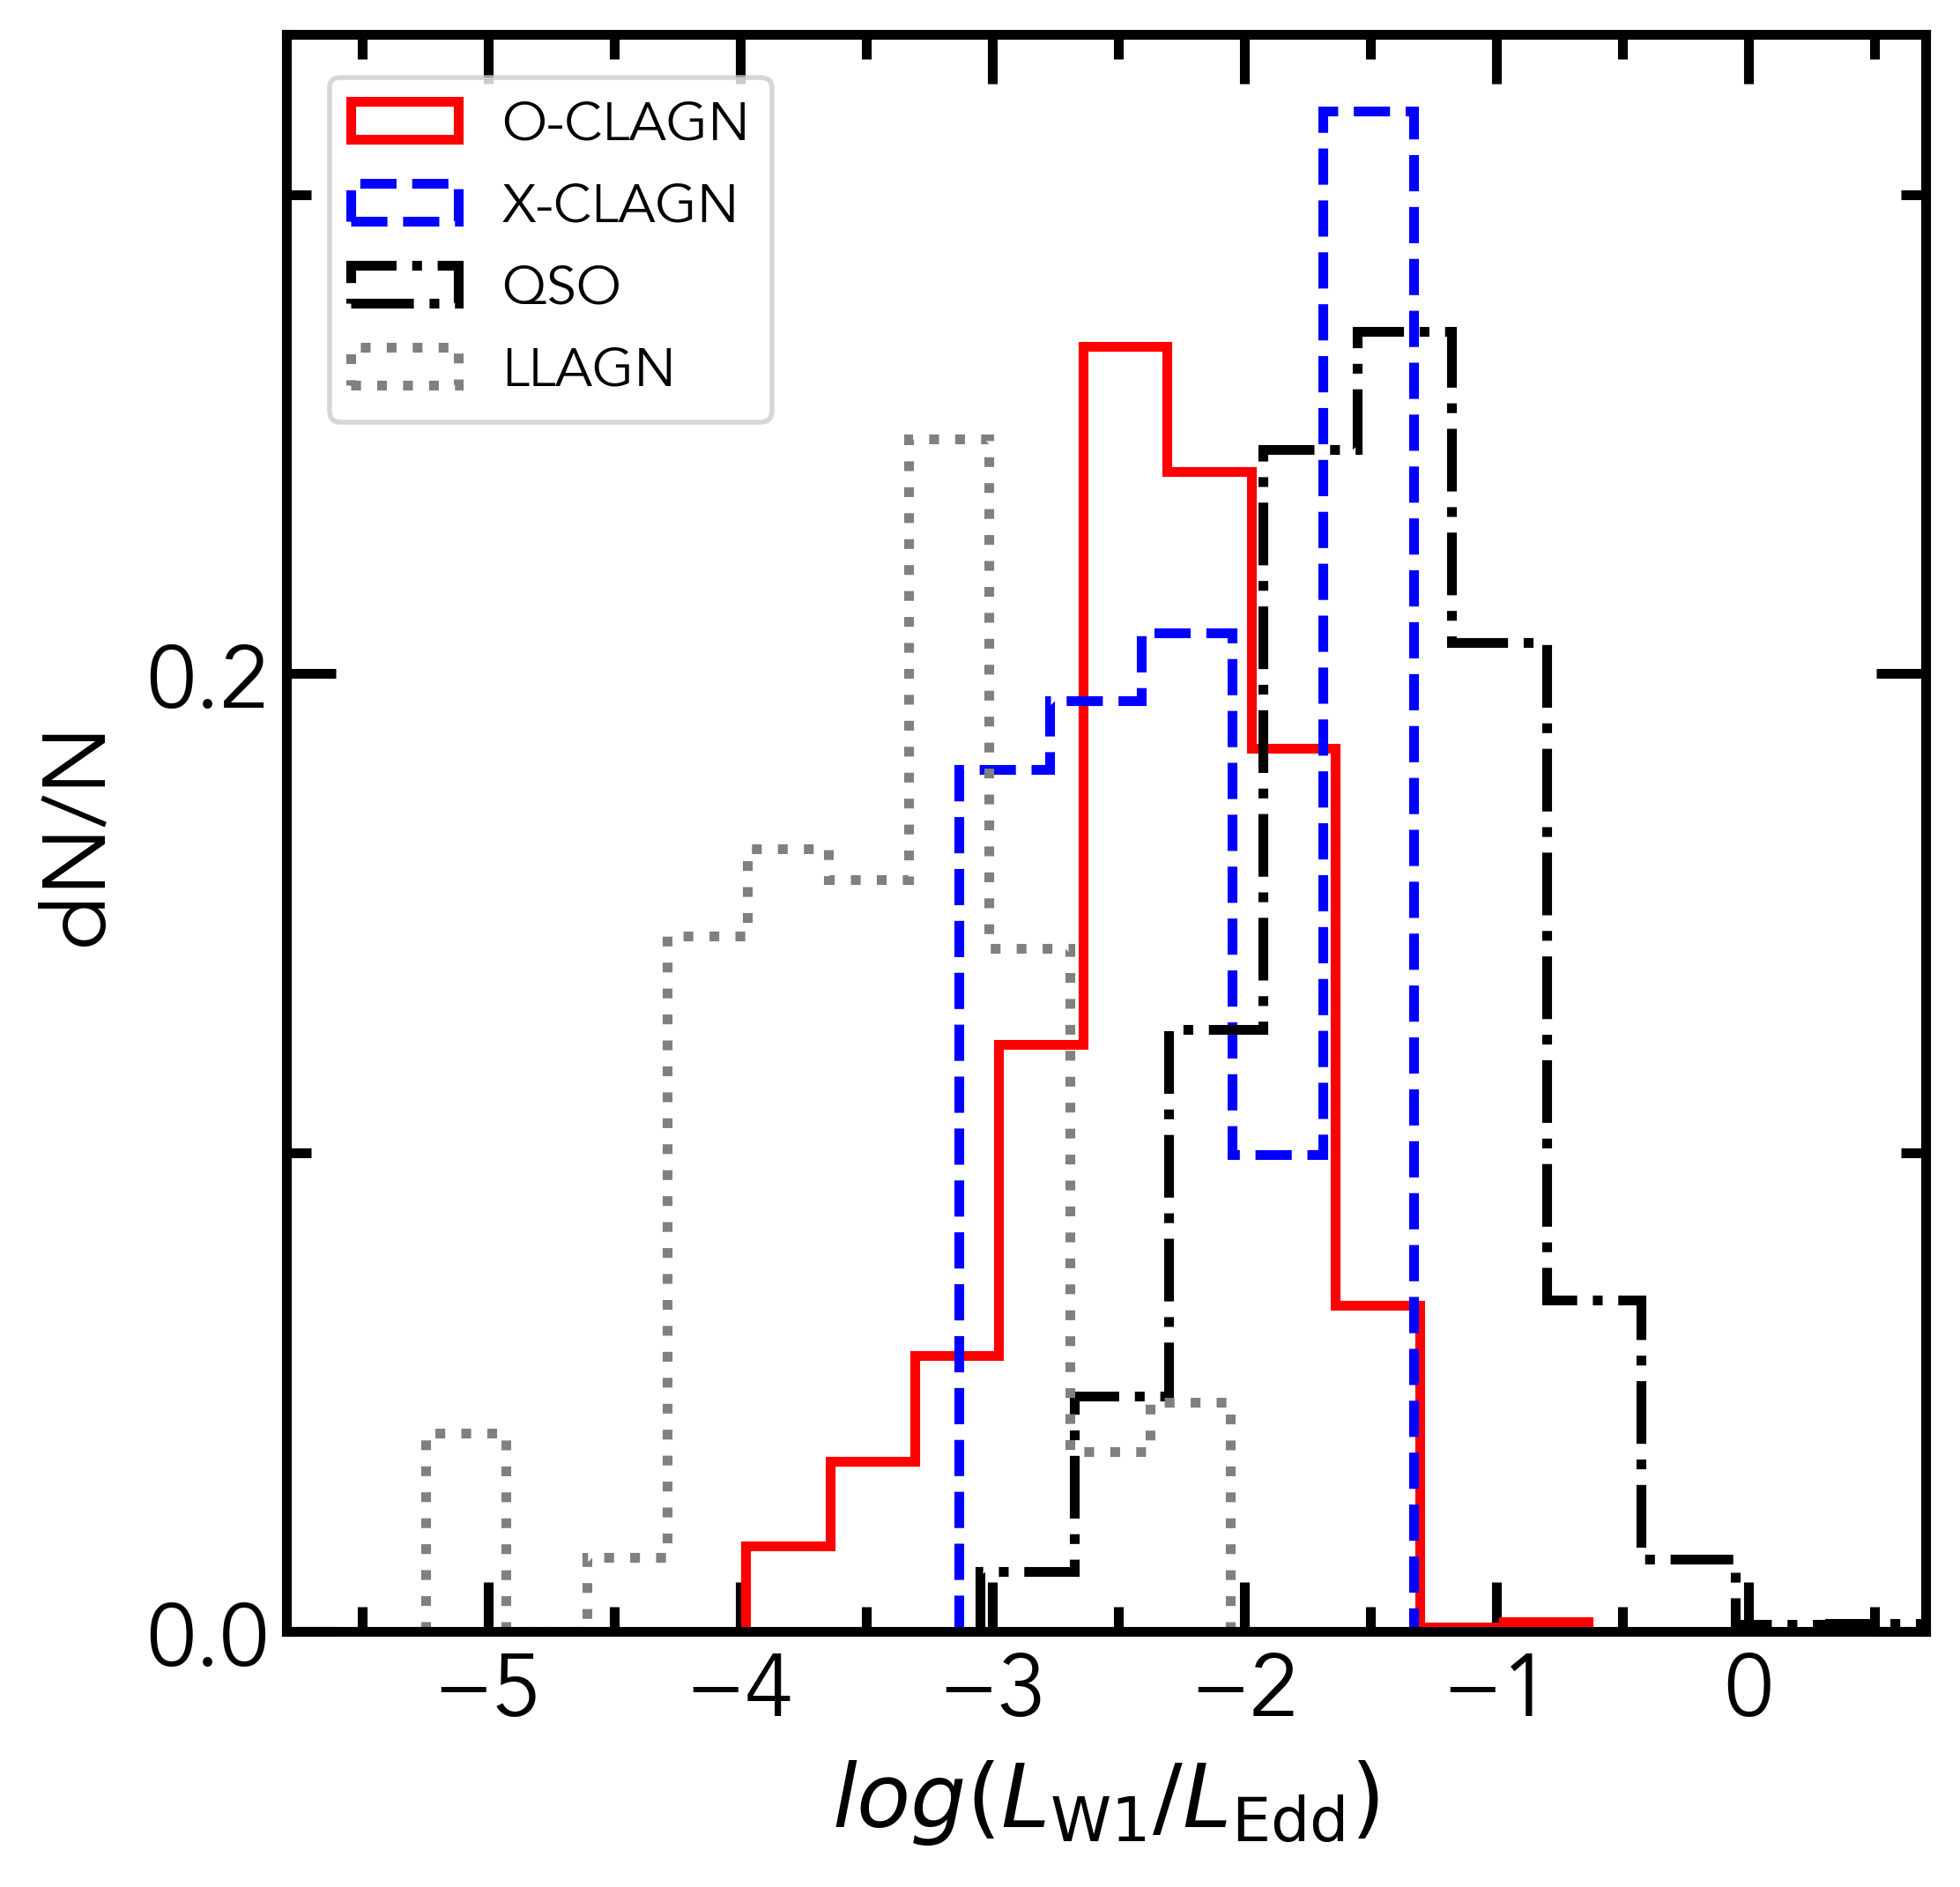
\includegraphics[width=0.5\textwidth]{pic/WISE_LW1_Ledd_hist_rebin_OX.png}
    \caption{Distribution of the Eddington-scaled $W1$ band luminosity re-binned in each visit for LLAGNs\citep{2009MNRAS.399..349G}, CLAGNs and QSOs \citep{2007ApJ...667..131G}. }
    \label{fig:distribution_ledd}
\end{figure}


%ASAS-SN \citep[][]{2018ATel11893....1D} data showed a brightening of NGC 1566 around September 2017, which is the brightest in July 2018. 

due to its high cadence-monitoring observations


slope=0.28+0.07−0.06 
intercept=2.12+0.05−0.05 
scatter=0.14+0.04−0.03
slope=0.28+0.06−0.06 
intercept=2.20+0.04−0.05 
scatter=0.15+0.05−0.03

slope=0.39+0.04−0.04 
intercept=2.19+0.05−0.06
scatter=0.23+0.02−0.02
slope=0.36+0.04−0.04 
intercept=2.29+0.06−0.05
scatter=0.22+0.02−0.02

slope=0.39+0.03−0.03 
intercept=2.18+0.03−0.03 
scatter=0.22+0.02−0.01
slope=0.37+0.03−0.03 
intercept=2.26+0.04−0.04
scatter=0.21+0.02−0.02

%More study on LLAGNs and low-luminosity CLAGNs should be performed in the future works to further test this issue.  
%where the transition of accretion mode may play a key role
